Completa el crucigrama:

\begin{minipage}{0.45\textwidth}
    \ifprintanswers
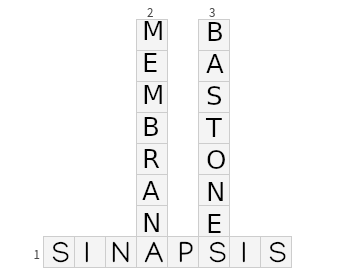
\includegraphics[width=0.9\linewidth]{../images/SINFI_U3_AC79_IMG1a.png}
\else
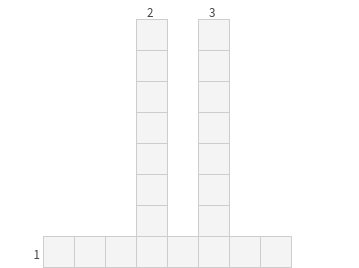
\includegraphics[width=0.9\linewidth]{../images/SINFI_U3_AC79_IMG1.png}
\fi
\end{minipage}\qquad
\begin{minipage}{0.35\textwidth}
    \begin{enumerate}
        \item Zona donde se conecta una neurona con otra.
        \item Permite el paso de iones positivos al interior y exterior de las neuronas en las células nerviosas.
        \item Células que se activan en la oscuridad o poca luz y perciben las intensidades luminosas entre el negro y el blanco.
    \end{enumerate}
\end{minipage}

